\subsubsection{Software System}

\paragraph{Communication System} \ \\
\vspace{-0.5cm}
Some communication system talk.


\paragraph{Graphical User Interface} \ \\
Our GUI prioritizes stability, usability, and responsiveness, balancing personalization with default configurations. Built with Python and PyQt5, it ensures a stable and efficient desktop experience.

\vspace{0.2cm}
\textbf{System Architecture}
The GUI follows a modular design, dividing functionality across four interfaces: Pilot, Copilot, Engineer, and Float. This enhances maintainability while tailoring tools to each role.

\vspace{0.2cm}
\textbf{Pilot Interface}
Designed for minimal clutter, the Pilot interface displays five camera feeds essential for navigation. To ensure smooth streaming, we use Python's \texttt{Multiprocessing} library, preventing latency and glitches. The Pilot can switch views and resize feeds as needed. Our redundant streaming system prevents a single point of failure—if one camera disconnects, others remain functional. 

\vspace{0.2cm}
\textbf{Copilot Interface}
The Copilot interface extends camera controls, allowing real-time brightness, contrast, and backlight adjustments for varying underwater conditions. It also displays telemetry data, including six degrees of freedom (Vx, Vy, Vz, Roll, Pitch, Yaw), depth, and thruster speeds, aiding in system monitoring and troubleshooting. A screenshot of the interface is shown in Figure \ref{fig:copilot_interface}.

\begin{figure}[ht]
    \centering
    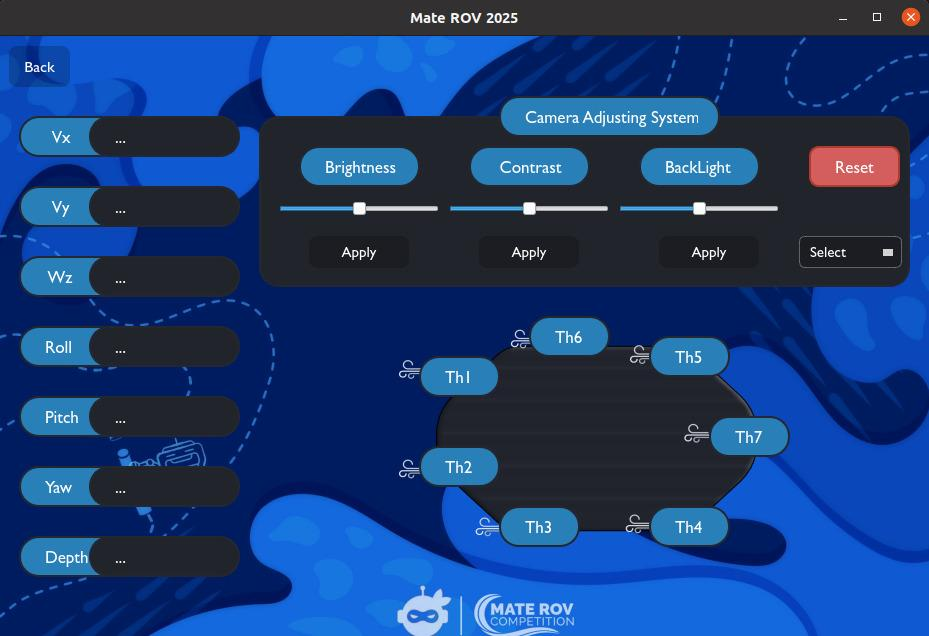
\includegraphics[width=0.8\columnwidth]{Sections/2Design Rationale/images/Copilot_interface.jpeg}
    \caption{Screenshot of the Copilot interface.}
    \label{fig:copilot_interface}
\end{figure}

\vspace{0.2cm}
\textbf{Engineer Interface}
The Engineer interface provides quick access to automation scripts for tasks like invasive carp detection and depth estimation. It also facilitates seamless media capture for Photosphere documentation. All functions are integrated within the GUI, streamlining workflow without external tools. A screenshot of the interface is shown in Figure \ref{fig:Engineer_interface}.

\begin{figure}[h]
    \centering
    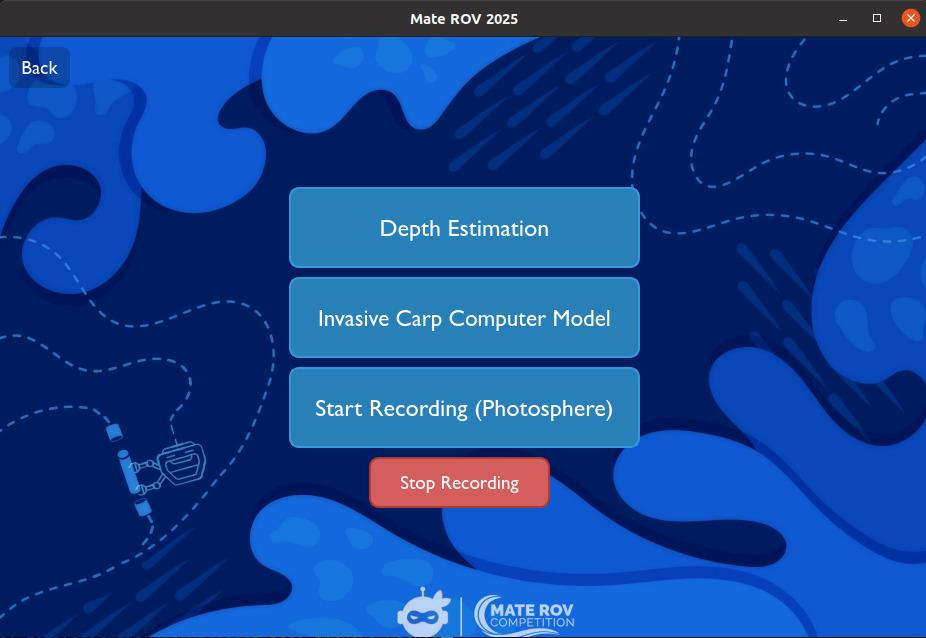
\includegraphics[width=0.8\columnwidth]{Sections/2Design Rationale/images/Engineer_interface.jpeg}
    \caption{Screenshot of the Engineer interface.}
    \label{fig:Engineer_interface}
\end{figure}

\vspace{0.2cm}
\textbf{Float Interface}
The Float interface enables communication with the float before vertical profiling begins and displays depth data along with additional metrics post-profile.


\paragraph{Some third point} \ \\
\vspace{-0.5cm}

some software system talk.